%%%%%%%%%%%%%%%%%%%%%%%%%%%%%%%%%%%%%%%%%%%%%%%%%%
\begin{frame}[fragile]{Standard Problem for Webapps?}

\begin{itemize}
\item Testing that frontend and backend play nicely together
\end{itemize}

\end{frame}

%%%%%%%%%%%%%%%%%%%%%%%%%%%%%%%%%%%%%%%%%%%%%%%%%%
\begin{frame}[fragile]{Standard Approach: ``Super-Na\"ive''}

\begin{itemize}
\item Backend develops API
\item Backend tests itself
\item Frontend waits until backend is implemented
\item Frontend tests itself and the interaction via integration tests
\end{itemize}

Problems:

\begin{itemize}
\item Frontend development is blocked
\item Integration tests are slow
\item Full integration testing does not scale
\end{itemize}


\end{frame}

%%%%%%%%%%%%%%%%%%%%%%%%%%%%%%%%%%%%%%%%%%%%%%%%%%
\begin{frame}[fragile]{Standard Approach: ``Still Quite Na\"ive''}

\begin{itemize}
\item Backend develops API
\item Backend tests itself
\item Frontend writes mocks for backend API
\item Frontend can be developed immediately
\item Frontend tests itself via mocks
\end{itemize}

Problems:

\begin{itemize}
\item Frontend relies on mocks for backend API
\item How to ensure that the mocks reflect the backend's actual behaviour?
\item Usually, backend behaviour changes
\item Frontend does not notice because mocks still look good
\end{itemize}

\end{frame}

%%%%%%%%%%%%%%%%%%%%%%%%%%%%%%%%%%%%%%%%%%%%%%%%%%
\begin{frame}[fragile]{Standard ``Industry-Strength'' Approach}

\only<1>{
\begin{itemize}
\item Consumer-Driven Contract Testing
\item Hand-written contracts
\end{itemize}
}

\only<2>{
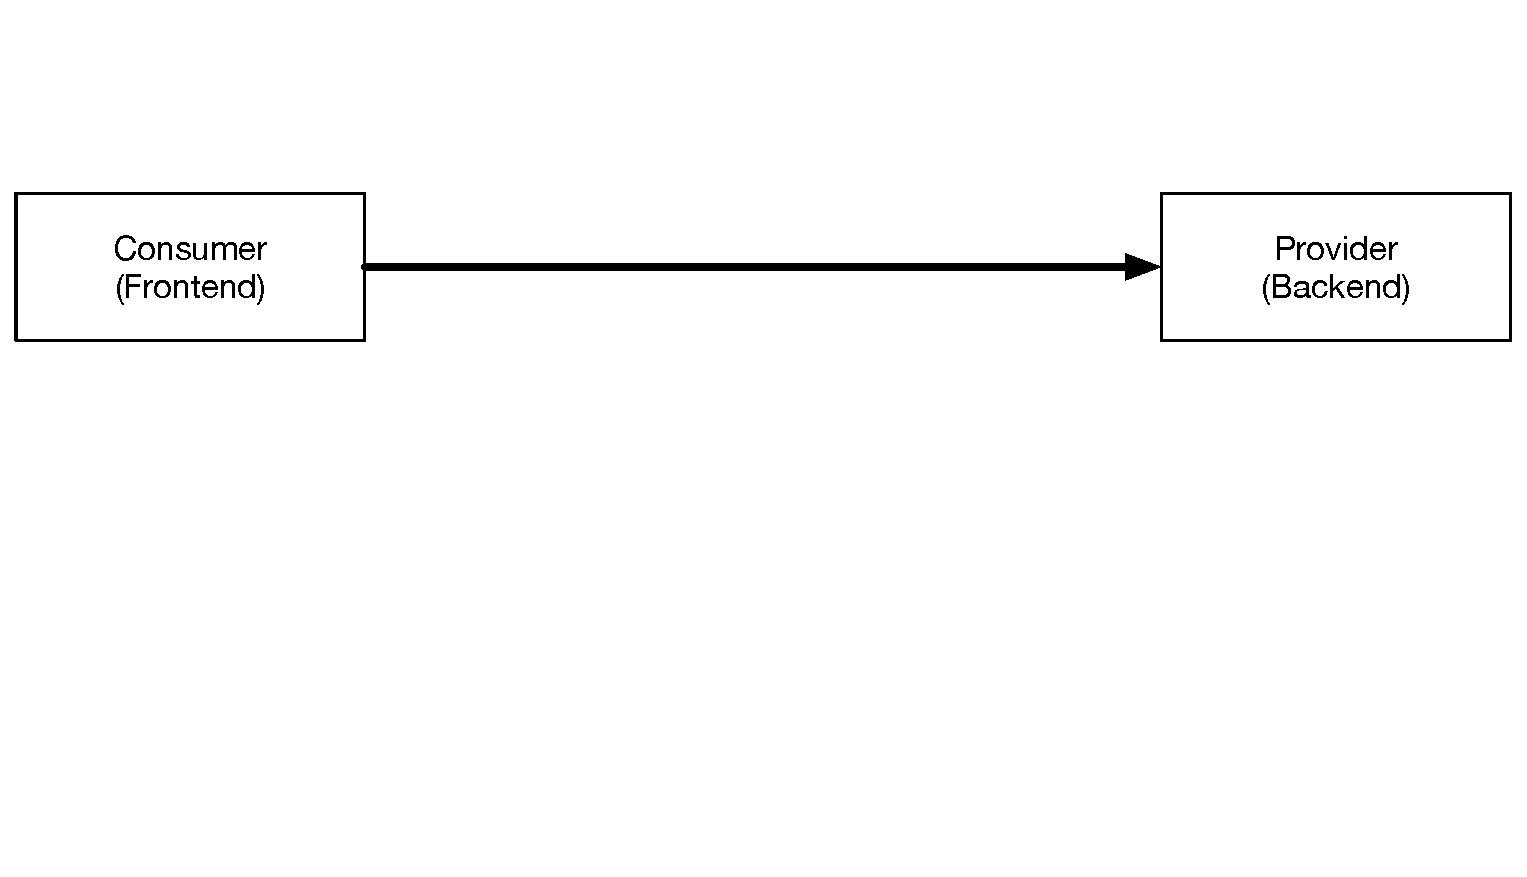
\includegraphics[width=\textwidth]{images/CDCT1.pdf}
}
\only<3>{
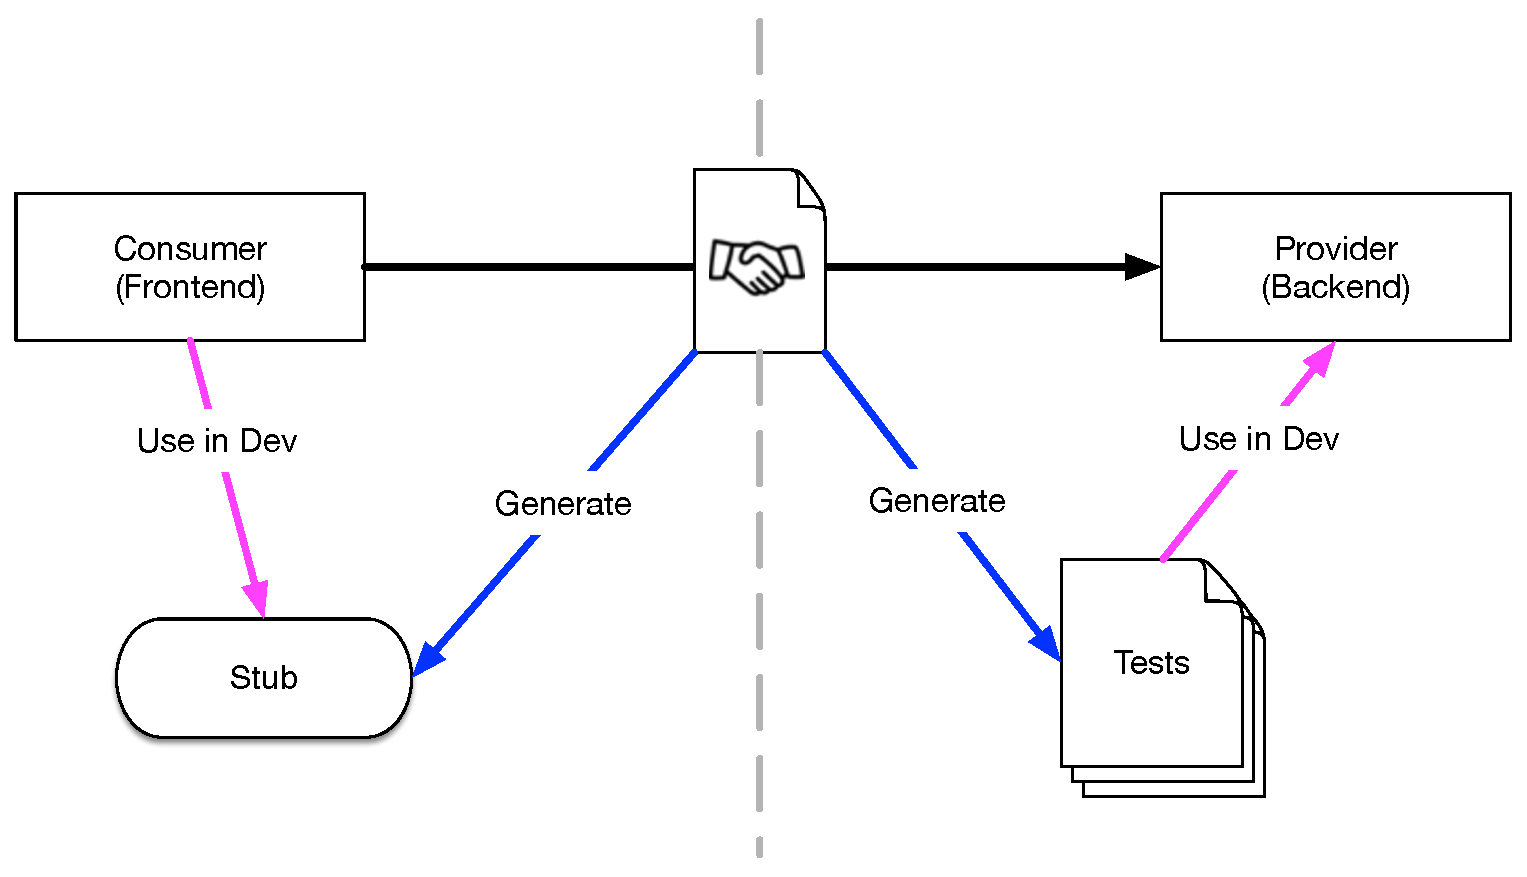
\includegraphics[width=\textwidth]{images/CDCT7.pdf}
}

\only<9>{
Problems:

\begin{itemize}
\item Contract testing is only as good as its contracts
\item Manual contract-writing can be tedious and even error-prone
\item Errors may only be discovered late in the process, when the backend implements some functionality and discovers that it does not match the contract
\item If contracts are too sparse, we miss out
\item If contracts are too verbose (or too many), testing takes too long
\end{itemize}
}

\end{frame}

%%%%%%%%%%%%%%%%%%%%%%%%%%%%%%%%%%%%%%%%%%%%%%%%%%
\begin{frame}[fragile]{Our ``formal model'' approach}

\begin{itemize}
\item Describe the Frontend-Backend integration in a formal model
\item Generate tests for the backend from this model
\item Generate mocks for the frontend from this model
\item Guarantee: All aspects (that are in the model) are covered by the tests and mocks
\end{itemize}

\end{frame}

%%%%%%%%%%%%%%%%%%%%%%%%%%%%%%%%%%%%%%%%%%%%%%%%%%
\begin{frame}[fragile]{}

\begin{itemize}
\item
\end{itemize}

\end{frame}

%%%%%%%%%%%%%%%%%%%%%%%%%%%%%%%%%%%%%%%%%%%%%%%%%%
\begin{frame}[fragile]{}

\begin{itemize}
\item
\end{itemize}

\end{frame}

%%%%%%%%%%%%%%%%%%%%%%%%%%%%%%%%%%%%%%%%%%%%%%%%%%
\begin{frame}[fragile]{}

\begin{itemize}
\item
\end{itemize}

\end{frame}

%%%%%%%%%%%%%%%%%%%%%%%%%%%%%%%%%%%%%%%%%%%%%%%%%%
\begin{frame}[fragile]{}

\begin{itemize}
\item
\end{itemize}

\end{frame}

%%%%%%%%%%%%%%%%%%%%%%%%%%%%%%%%%%%%%%%%%%%%%%%%%%
\begin{frame}[fragile]{}

\begin{itemize}
\item
\end{itemize}

\end{frame}

